\textbf{Colour Choice:}
In order to make the program more appealing, colours are used in the design. It is important that the colours give the right statement, and that they seem attractive to the user.

The colour that was discussed first, using Paletton, was a red colour. This was supposed to be the colour of headlines and such, in the program. The reason for discussing red is that red indicates appetite and food\cite{color_psychology}. Red was not chosen though, as it is too strong of a colour which can also indicate danger or alerts.

Since red was not the optimal choice of colour, orange was considered for its similarity to red. Orange has the same quality of red to encourage appetite for the user. Furthermore is orange also a cheerful colour, and it was found to be very appealing, lastly it may be used in the program without standing out too much, or give the user wrong impressions.

\begin{figure}[H]
	\centering
    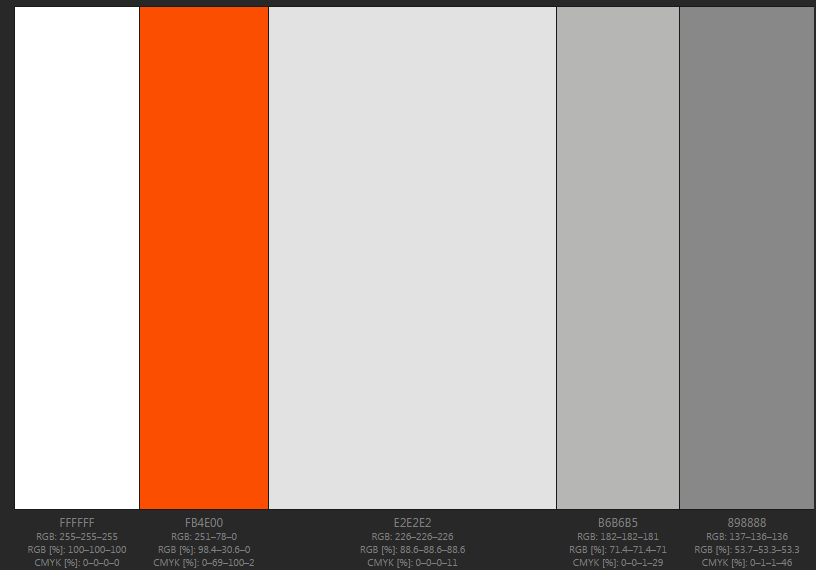
\includegraphics[width=\textwidth, clip=true, trim=0cm 0cm 0cm 8cm]{Grafik/FoodPlanner/ChosenColours}
	\caption{The chosen colours for the software.}
	\label{ChosenColours}
\end{figure}
The shade of orange and a range of gray colours were chosen, and can be seen in \cref{ChosenColours}.

The colour \#898888 is used for the borders of the program. If something is parted, or a button needs a border, this colour is used. The reason for choosing this colour is that it is much darker than the other colours and gives a clear indication of an ending item.

The colour \#FB4E00 is the orange colour as can be seen in \cref{ChosenColours}. This colour is the one used for the headline text, as is the main colour of the program, since it is the only colour that cannot be characterized as a neutral colour. It is only used for the headline text, as it would be difficult for the user to read the text if it was all orange.

The colour \#E2E2E2 is used for the background of the software. This is a very light colour, and it is easy to read black text on it, furthermore does the orange headlines stand more sharp, which makes them easier to see. Therefore this colour was chosen for the background. The white colour \#FFFFFF was also considered, but it was too light, and might irritate the user, lastly it did not go as well with the borders as \#E2E2E2.

